% Copyright 2004 by Till Tantau <tantau@users.sourceforge.net>.
%
% In principle, this file can be redistributed and/or modified under
% the terms of the GNU Public License, version 2.
%
% However, this file is supposed to be a template to be modified
% for your own needs. For this reason, if you use this file as a
% template and not specifically distribute it as part of a another
% package/program, I grant the extra permission to freely copy and
% modify this file as you see fit and even to delete this copyright
% notice. 

\documentclass{beamer}

% There are many different themes available for Beamer. A comprehensive
% list with examples is given here:
% http://deic.uab.es/~iblanes/beamer_gallery/index_by_theme.html
% You can uncomment the themes below if you would like to use a different
% one:
%\usetheme{AnnArbor}
%\usetheme{Antibes}
%\usetheme{Bergen}
%\usetheme{Berkeley}
%\usetheme{Berlin}
%\usetheme{Boadilla}
%\usetheme{boxes}
%\usetheme{CambridgeUS}
%\usetheme{Copenhagen}
%\usetheme{Darmstadt}
%\usetheme{default}
%\usetheme{Frankfurt}
%\usetheme{Goettingen}
%\usetheme{Hannover}
%\usetheme{Ilmenau}
%\usetheme{JuanLesPins}
%\usetheme{Luebeck}
\usetheme{Madrid}
%\usetheme{Malmoe}
%\usetheme{Marburg}
%\usetheme{Montpellier}
%\usetheme{PaloAlto}
%\usetheme{Pittsburgh}
%\usetheme{Rochester}
%\usetheme{Singapore}
%\usetheme{Szeged}
%\usetheme{Warsaw}







\title{Relieving the Space Jam}

% A subtitle is optional and this may be deleted
\subtitle{Assessment of a Quick-Response Satellite Mission to Neutralize Debris from Orbital Fragmentation Events}

\author{*Matthew Moreno, *Becky Hanscam, Caleb Spring \\{\small Advisor: Carl Toews}}

% - Give the names in the same order as the appear in the paper.
% - Use the \inst{?} command only if the authors have different
%   affiliation.

\institute[University of Puget Sound] % (optional, but mostly needed)
% - Use the \inst command only if there are several affiliations.
% - Keep it simple, no one is interested in your street address.

\date{Math Day | April 30th, 2016}
% - Either use conference name or its abbreviation.
% - Not really informative to the audience, more for people (including
%   yourself) who are reading the slides online

\subject{Mathematical Competition in Modeling}
% This is only inserted into the PDF information catalog. Can be left
% out. 

% If you have a file called "university-logo-filename.xxx", where xxx
% is a graphic format that can be processed by latex or pdflatex,
% resp., then you can add a logo as follows:

% \pgfdeclareimage[height=0.5cm]{university-logo}{university-logo-filename}
% \logo{\pgfuseimage{university-logo}}

% Delete this, if you do not want the table of contents to pop up at
% the beginning of each subsection:
\AtBeginSection[]
{
  \begin{frame}<beamer>{Outline}
    \tableofcontents[currentsection,hideallsubsections]
  \end{frame}
}

% Let's get started
\usepackage{geometry}
\usepackage{pageslts}
\usepackage{amsmath,amssymb,amsthm}
\usepackage{ textcomp }
\usepackage{graphicx}
\usepackage{float}
\usepackage{hyperref}

\begin{document}


\begin{frame}
  \titlepage
\end{frame}

\begin{frame}{Outline}
  \tableofcontents[hideallsubsections]
  % You might wish to add the option [pausesections]
\end{frame}

% Section and subsections will appear in the presentation overview
% and table of contents.
\section{The Mathematical Competition in Modeling}

\subsection{Question}

\begin{frame}{The Competition}
    What is the MCM?
    \begin{itemize}
     \item {3 person teams}
     \item {Choose 1 of 3 posed questions}
     \item {Answer the question to best of your abilities}
     \item {4 days}
    \end{itemize}\\
  %sounds easy right? Wrong.

    Who does it?
     \begin{itemize}
         \item {High school and college students}
         \item {95 \% foreign teams (mostly China)}
         \item {\textbf{Honorable Mention}: top 45\% of 1453 teams}
     \end{itemize}\\
  
\end{frame}

\subsection{Timeframe}

% You can reveal the parts of a slide one at a time
% with the \pause command:
\begin{frame}{Problem B: Space Junk}
"Develop a time-dependent model to determine the best alternative or combination of alternatives
that a private firm could adopt as a commercial opportunity to address the space debris problem."
  \begin{itemize}
  \item {Quantitative analysis of costs, risks, benefits, etc.}
  \item {Assess independent alternatives}
  \item {Address "What if?" scenarios}
  \item {Determine if an economically attractive opportunity exists}
  \item {Compare the different debris removal options}
  \item {Provide a specific recommendation as to how the debris should be removed}
  \item {Provide innovative alternatives for avoiding collisions}
  \item {Recommend a particular action, combination of actions,
or no action}
  \end{itemize}
\end{frame}

\begin{frame}{Problem B: Space Junk}
"Develop a time-dependent model to determine the best alternative or combination of alternatives
that a private firm could adopt as a commercial opportunity to address the space debris problem."
  \begin{itemize}
  \item {Quantitative analysis of costs, risks, benefits, etc.}
  \item {\textbf{Assess independent alternatives}}
  \item {Address "What if?" scenarios}
  \item {Determine if an economically attractive opportunity exists}
  \item {Compare the different debris removal options}
  \item {Provide a specific recommendation as to how the debris should be removed}
  \item {\textbf{Provide innovative alternatives for avoiding collisions}}
  \item {Recommend a particular action, combination of actions,or no action}
  \end{itemize}
\end{frame}

\section{Space Junk}

\subsection{What is Space Junk?}

\begin{frame}{What is Space Junk?}
Thousands of man-made objects have reached space since the mid 1900's \cite{ODPO} \\
% satellites, shuttles and probes
\(\Rightarrow{}\) Uncontrolled debris when:
    \begin{itemize}
        \item{End of functional lifespan}
        \item{Become unresponsive}
    \end{itemize}
\(\Rightarrow{}\) Debris remains in orbit until gravity pulls it into Earth's atmosphere:\\
\hspace{10mm} \rightarrow \textbf{Drag} \rightarrow \textbf{Deceleration} \rightarrow \textbf{De-orbited} \rightarrow \textbf{DESTROYED!}\\
\begin{center}
\(\dotsc{}\) but very slowly\\
%many years to occur naturally, depends on altitude,
\end{center}
\(\Rightarrow{}\) Amount of debris is \textbf{rapidly growing}!\\
\(\Rightarrow{}\) Many explosions and collisions, each one creating dust clouds with many smaller fragments traveling at very high velocities \cite{UN}.\\
 \begin{itemize}
  \item {
    Video: Individual Collision \url{https://youtu.be/9cd0-4qOvb0?t=4m24s}
    % stop at 4:51
  }
  \end{itemize}
\end{frame}

 
\subsection{Why it's Bad}

% You can reveal the parts of a slide one at a time
% with the \pause command:
\begin{frame}{Why it's Bad}

To illustrate, 1 kg object moving at normal low earth orbit speeds packs the punch of a 35,000 kg truck moving at 190 km/h \cite{punch}!\\
\(\Rightarrow{}\) \textbf{Cascading effect}, as each piece of debris poses the risk of damage.
 \begin{itemize}
  \item {
     Video: Domino Effect \url{https://youtu.be/9cd0-4qOvb0?t=5m44s}
     % stop at 6:26
  }
 \end{itemize}
\(\Rightarrow{}\) At the end of the 20th century, over \textbf{35 million pieces of debris} were present in Earth's orbit \cite{1995 IA}.
   %This number is growing exponentially, and with it grows the probability of damage to functional spacecraft \cite{UN}.
  \begin{itemize}
      \item{approximately \(72\% \) of cataloged debris is in the Lower Earth Orbit (\(< 2000\) km \cite{1995 IA})}
      %total takes into account the debris smaller than 10 cm that is statistically estimated by damage to spacecraft because it is too small to be seen by radar
      \item{LEO contains the highest concentrations of debris at a density of \textbf{\(4.55 \times 10^{-8}\) debris fragments per cubic kilometer} and most concentrated around \textbf{900 km} altitude \cite{fragments}}
  \end{itemize}

\end{frame}

\subsection{What to Do About It}

% You can reveal the parts of a slide one at a time
% with the \pause command:
\begin{frame}{What to Do About It}
  \begin{itemize}
  \item {
    solar sail-type debris net 
  }
  \item {   
    gas puffs
  }
  \item {
    lasers
  }
  \item {
   and many other ideas...
  }

  \end{itemize}
\end{frame}


\section{The Quick Response Mission Concept}

\subsection{Overview}

\begin{frame}{The Quick Response Mission Concept}
 \begin{block}{The Idea}
Launch a quick-response mission to target fragmentation and collision events soon after they occur.
\end{block}
  The Idea: 
  \begin{itemize}
  \item{SORES: Space Orbit REmoval Satellite
  }
  \item {
    orbit in the same orbit that the satellite occupied, in the reverse direction
  }
  \item {
    deorbit all debris that it comes within a certain distance of (the "effective radius") through... some mechanism
  }
  \end{itemize}
\end{frame}



\section{Our Model}

\subsection{The Mathematical Foundation}

\begin{frame}{Modeling Foundation: Orbital Mechanics}
 \begin{block}{The Idea}
 Use standard classical physics concepts and Euler's method to propagate the position of an object over time to simulate its orbit.
\end{block}
\small{
\begin{itemize}
 \item{We approximate the system to a 1st order set of differential equations by updating a vector \(U(t)\) of initial conditions.}

\item{Apply the equation of force on mass \(m\) a distance \(d\) from a second mass \(M\), 
\begin{align}
F_{g} = GM \frac{m}{d^3} \vec{r}.
\end{align} }
\item{Use Euler's method (explicit scheme) to solve the initial value problem of
\begin{align}
\vec{x}' = F_{g}(t,U).
\end{align} }
\item{Propagate the position and velocity over the time interval to trace the orbit of the object.}
\end{itemize}

}

\end{frame}

% \begin{frame}{Modeling Foundation: Picking an Orbit}
% \begin{block}{The Idea}
% Put satellite into a stable orbit.
% \end{block}
% \small{
%  A satellite in stable orbit experiences balanced centripetal and gravitational forces, so
% \begin{align}
% \frac{GM_{s}M_{E}}{r^2} = M_{s}r\omega^2 \rightarrow
%  \bar{v} = \sart{\frac{G M_{E}}{r}}
% \end{align}
% We must orient its velocity perpendicular to the surface of the Earth. We solve
% \begin{align}
% \langle \mathring{v}_x, \mathring{v}_y \rangle &= - \langle x_x, x_y \rangle \\
% 0 &= \langle x_x, x_y, x_z \rangle \cdot \langle \mathring{v}_x,\mathring{v}_y,\mathring{v}_z \rangle \\
% \mathring{\vec{v}} &= <-x_x, -x_y, \sqrt{x_x^2 + x_y^2}>.
% \end{align}
% Putting this information together,
% \begin{align}
% \vec{v} = \frac{\mathring{\vec{v}}}{||\vec{\mathring{v}}||} \cdot \bar{v}.
% \end{align}

% }
% \end{frame}

\begin{frame}{Modeling Foundation: Fragmentation Events}
\begin{block}{The Idea}
We assume that all the energy generated in the fragmentation event is released as kinetic energy in random directions to equally sized fragments.
\end{block}

\begin{align}
J = \sum_{i = 0}^{n} \mathit{\mathit{KE}}_{i} = n \frac{1}{2} m_{i}\bar{v_{i}}^2.
\end{align}
Solving for $\bar{v_{i}}$ yields
\begin{align}
\bar{v_{i}} = \sqrt{2 J / m_{i}}.
\end{align}
We assume that fragments disperse in random directions. Thus, with $\vec{u_{i}}$ as a unit vector with random orientation, the velocity vector of the $i$th debris fragment, $\vec{v_i}$ is given as
\begin{align}
\vec{v_{i}} = \vec{v_{s}} + \bar{v_{i}} \vec{u_i}.
\end{align}

\end{frame}


\subsection{Sensitivity Analysis}

% You can reveal the parts of a slide one at a time
% with the \pause command:
\begin{frame}{Amount of Debris}
\begin{figure}
\begin{center}
\label{fig:debrisfragmentssensitivity}
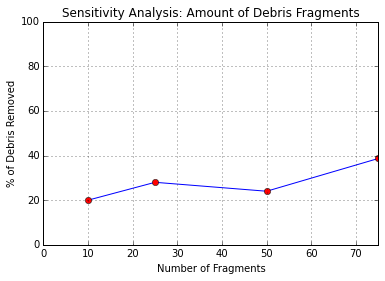
\includegraphics[width=0.7\textwidth]{fragments.png}\\
\stepcounter{figure}
Figure \arabic{figure}: Results of sensitivity analysis of the performance of SORES predicted by our model to the number of debris generated in the orbital fragmentation event.
\end{center}
\end{figure}
\end{frame}

\begin{frame}{Explosion Energy}
\begin{figure}
\begin{center}
\label{fig:explosionenergysensitivity}
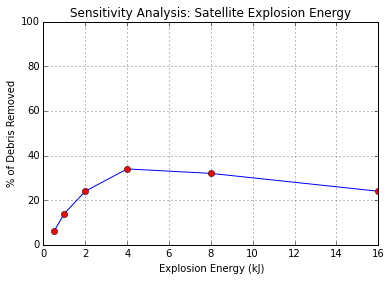
\includegraphics[width=0.7\textwidth]{energy.png}\\
\stepcounter{figure}
Figure \arabic{figure}: Results of sensitivity analysis of the performance of SORES predicted by our model to the energy released in the orbital fragmentation event.
\end{center}
\end{figure}
\end{frame}

\begin{frame}{Iterations of Numerical Approximation}
\begin{figure}
\begin{center}
\label{fig:iterationsensitivity}
\stepcounter{figure}
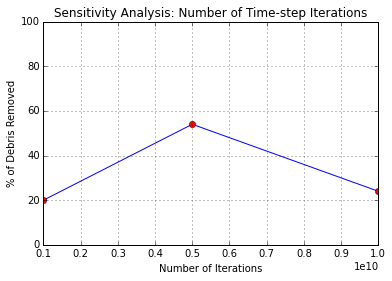
\includegraphics[width=0.7\textwidth]{iterations.png}\\
Figure \arabic{figure}: Results of sensitivity analysis of the performance of SORES predicted by our model to the number of iterations of each time-step.
\end{center}
\end{figure}
\end{frame}

\subsection{Model Assessment}
% \begin{frame}{Model Assessment: Visual}
% \begin{figure}
% \begin{center}
% \label{fig:unexploded_sat_orbit}
% 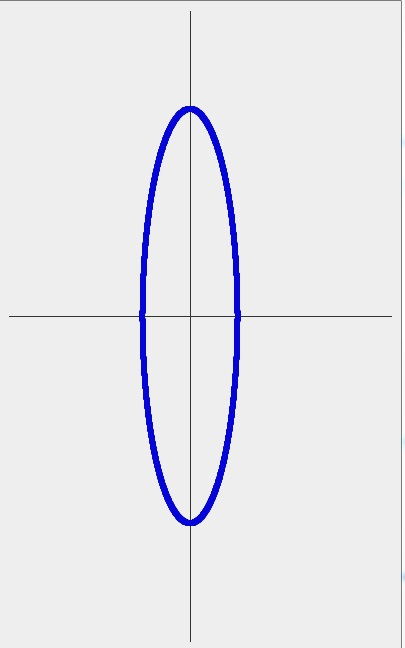
\includegraphics[width=0.3\textwidth]{side_regular_orbit_1.jpg}
% 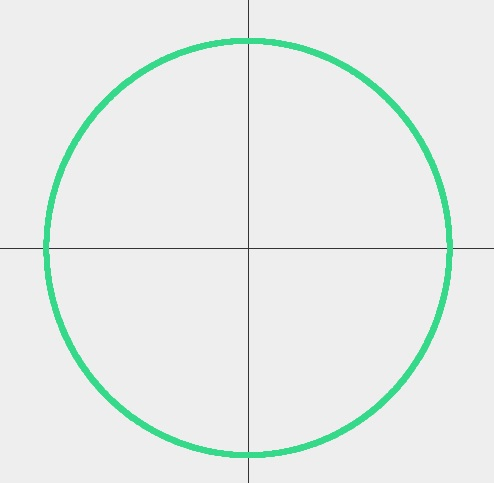
\includegraphics[width=0.3\textwidth]{side_regular_orbit_2.jpg}
% 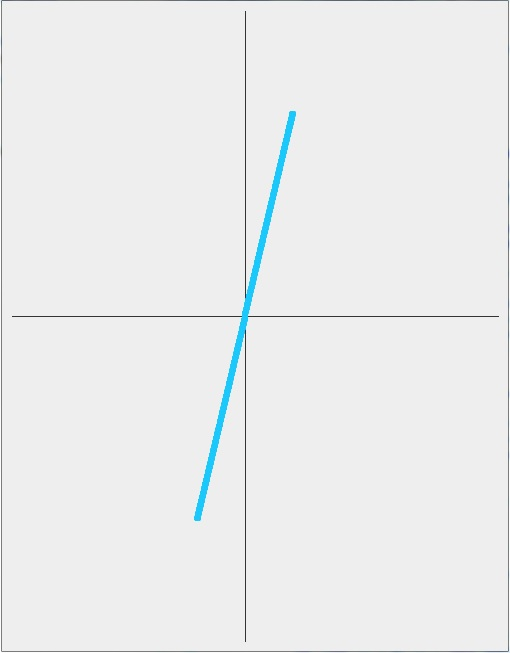
\includegraphics[width=0.3\textwidth]{top_regular_orbit.jpg}\\
% \stepcounter{figure}
% Figure \arabic{figure}: Side and top views of paths traced by an unexploded satellite in orbit.

% \end{center}
% \end{figure}
% \end{frame}

\begin{frame}{Model Assessment: Visual}
\begin{figure}
\begin{center}
\label{fig:sat_orbit_explosion}
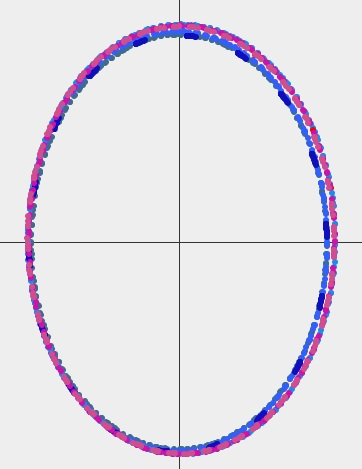
\includegraphics[width=0.4\textwidth]{depth.jpg}
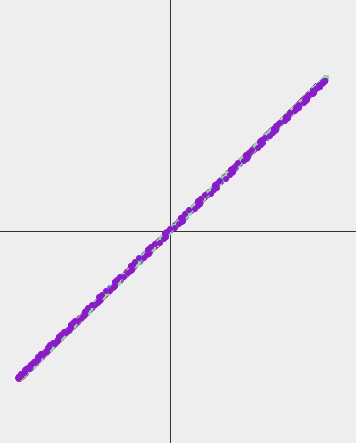
\includegraphics[width=0.4\textwidth]{top.jpg}\\
\stepcounter{figure}
Figure \arabic{figure}: Side and top views of paths traced by orbital debris after a 2 kJ fragmentation event.
\end{center}
\end{figure}
\end{frame}

\begin{frame}{Model Assessment: Conservation of Energy}
\begin{block}{The Idea}
Assess numerical approximation accuracy by looking at conservation of energy.
\end{block}

The total energy of each fragment can be given as 
\begin{align*}
E_{i} 
&= \mathit{KE}_{i} + \mathit{PE}_{i} \\
&= \frac{1}{2} m_{i} \bar{v_{i}}^2 - \frac{G M_{E} m_{i}}{r}
\end{align*}
where $m_{i}$ is the mass of the $i$th debris fragment.

\begin{itemize}
\item $N = 1\times10^{8}$ and $\ \Delta t = 7$ days $\rightarrow$ $2.0 \pm 1.7 \%$ fluctuation in total energy of each fragment.
\item  $N = 1\times10^{10}$ and $\Delta t = 100$ $\rightarrow$ $11.9 \pm 2.7 \%$ fluctuation in total energy of each fragment.
\end{itemize}

\end{frame}


\begin{frame}{Model Assessment: Strengths}

\begin{itemize}
        \item The model simulates orbital mechanics to an adequate accuracy, as assessed by visual analysis of orbit path and mathematical evaluation of conservation of energy in the model.
        \item The model provides a simple, but reasonable, simulation of satellite fragmentation in three dimensions over a short time period.
        \item The model successfully assesses the number of debris de-orbited by a SORES satellite, with this success count responding to changes in parameters (such as SORES effective radius and delay before SORES launch) as would be expected.
    \end{itemize}
    
\end{frame}

\begin{frame}{Model Assessment: Weaknesses}
 \begin{itemize}
        \item The model is computationally intensive, with computational costs scaling linearly both with number of fragments and mission duration. These costs make long-term simulation of large numbers of debris infeasible.
        \item The model neglects drag effects, the non-uniformity of Earth's gravitational field, and the gravitational interference of other celestial bodies. These effects are negligible for simulations of short time-periods, but their absence may affect longer term simulations.
        \item Most experimental results were derived from a single trial, which casts some uncertainty on their reproducibility.
    \end{itemize}
\end{frame}



\section{Results}

\subsection{Time Delay to Launch}

\begin{frame}{Time Delay to Launch}
\begin{figure}
\begin{center}
\label{fig:resultsvslaunchdelay}
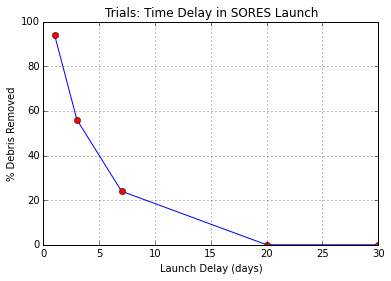
\includegraphics[width=0.7\textwidth]{delay.png}\\
\stepcounter{figure}
Figure \arabic{figure}: The performance of SORES, as measured by percent debris de-orbited, tabulated over several fragmentation-to-launch delays.
\end{center}
\end{figure}
\end{frame}


\subsection{SORES Effective Radius}

% You can reveal the parts of a slide one at a time
% with the \pause command:
\begin{frame}{SORES Effective Radius}
\begin{figure}
\begin{center}
\label{fig:resultsvseffectiveradius}
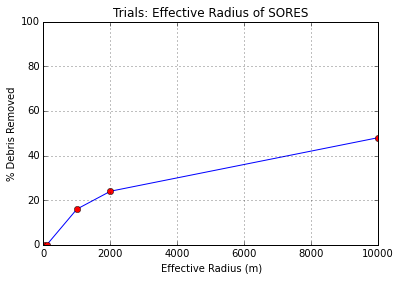
\includegraphics[width=0.7\textwidth]{radius.png}\\
\stepcounter{figure}
Figure \arabic{figure}: The relationship of SORES effective radius and its success at de-orbiting space debris.
\end{center}
\end{figure}
\end{frame}


\subsection{Orbital Altitude}

% You can reveal the parts of a slide one at a time
% with the \pause command:
\begin{frame}{Orbital Altitude}
\begin{figure}
\begin{center}
\label{fig:altitudesensitivity}
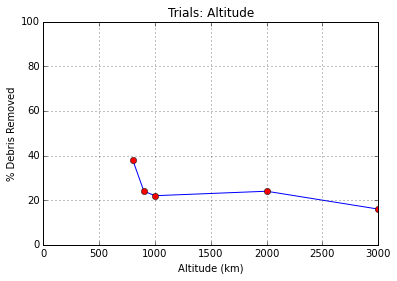
\includegraphics[width=0.7\textwidth]{altitude.png}\\
\stepcounter{figure}
Figure \arabic{figure}: SORES performance tabulated over a orbital altitudes ranging from LEO to mid MEO.
\end{center}
\end{figure}
\end{frame}

\section{Recommendations}

\subsection{Risks and Costs}

% You can reveal the parts of a slide one at a time
% with the \pause command:
\begin{frame}{Risks and Costs}
  \begin{block}{The Idea}
 A SORES approach to space junk removal simply does not pen out as a profitable endeavor at this time, but might be viable if costs go down and the space junk problem gets worse.
\end{block}
  \begin{itemize}
  \item {
    Designing and launching a mission is expensive: \$290 million + \cite{cost}
  }
  \item {   
   Insurance companies cover satellites for an average of \(\$129\) million for catastrophic failure events, including damage from debris \cite{cost}
  }
  \end{itemize}
  \pause
  Bounty of \$2,050 on each debris fragment, calculated using...
  \begin{itemize}
    \item{
   The probability of a collision between a satellite and a debris fragment in a year
  }
  \item {   
    The number of satellites with orbits passing through the LEO
  }
\item {   
    The approximate number of debris fragments in the LEO
  }
  \end{itemize}
  \begin{center}
   \(\Rightarrow{}\) 4880 debris fragments per mission
  \end{center}
 
\end{frame}

\begin{frame}{Recommendations}
 \begin{itemize}
    \item SORES needs to be maneuverable and/or structurally robust to impact with debris
    \pause
    \item Our models predict that SORES type missions are more successful at remedying low-altitude fragmentation events... a SORES mission is more likely to pencil out for a low-altitude fragmentation event.
    \pause
    \item To maximize the effectiveness of a SORES mission, minimizing the time that passes between a fragmentation event and launch is key.
    \pause
    \item The effectiveness of a SORES mission also depends on the effective radius of debris capture. This radius should be, at a minimum, around 1 km.
    \pause
    \item Our cost assessments suggest that a SORES-type intervention is not currently economically feasible. However, if the space debris situation deteriorates significantly, this type of intervention may become palatable.
\end{itemize}
\end{frame}

% All of the following is optional and typically not needed. 
\appendix
\section<presentation>*{\appendixname}
\subsection<presentation>*{For Further Reading}

\begin{frame}[allowframebreaks]
  \frametitle<presentation>{For Further Reading}
    
  \begin{thebibliography}{10}
    
  \beamertemplatebookbibitems

\tiny{
 \bibitem{1995 IA} 
United States. Office of Science and Technology Policy. Transportation Research and Development. \textit{Interagency Report on Orbital Debris 1995}. NASA Orbital Debris Program Office. Web. 29 Jan. 2016.
\bibitem{ESA} 
"Space Debris." \textit{European Space Agency}. 19 Apr. 2013. Web. 31 Jan. 2016.
\bibitem{ODPO}
\textit{"NASA Orbital Debris Program Office."} NASA Orbital Debris Program Office. Web. 29 Jan. 2016.
\bibitem{solar cycle}
Hathaway, Dr. David. "Solar Cycle Prediction." \textit{Solar Physics}. Marshall Space Flight Center and NASA, 12 Jan. 2016. Web. 29 Jan. 2016.
\bibitem{UN}
United Nations. \textit{Technical Report on Space Debris}. NASA Orbital Debris Program Office, 1999. Web. 29 Jan. 2016.
\bibitem{excel}
\textit{UCS Satellite Database 9-1-15.} Union of Concerned Scientists, 1 Sept. 2015. Excel.
\bibitem{punch}
Redd, Nola Taylor. "Space Junk: Tracking \& Removing Orbital Debris." \textit{Space.com}. 8 Mar. 2013. Web. 31 Jan. 2016.
\bibitem{model}
Bordovitsyna, T. V., and A. G. Aleksandrova. "Numerical Modeling of the Formation, Orbital Evolution, and Distribution of Fragments of Space Debris in Near-Earth Space." \textit{Solar System Research} 44.3 (2010): 238-51. Web. 30 Jan. 2016.
\bibitem{boom}
Pardini, C., L. Anselmo, A. Rossi, A. Cordelli, P. Farinella. \textit{The 1997.0 CNUCE Orbital Debris Reference Model.} 8th AAS/AIAA Space Flight Mechanics Meeting, 1997. Web. 29 Jan. 2016. 
\bibitem{fragments}
United States. NASA. Orbital Debris Program. \textit{History of On-Orbit Satellite Fragmentations}. NASA Orbital Debris Program Office, June 2008. Web. 29 Jan. 2016.
\bibitem{cost}
Miller, David W., John Keesee, and Cyrus Jilla. \textit{Space Systems Cost Modeling.} Massachusetts Institute of Technology, Sept. 2003. PPT.
\bibitem{risk}
Bensoussan, Denis. \textit{Satellite Vulnerability to Space Debris Risk.} Dubai: World Space Risk Forum, 2012. PPT.
\bibitem{cost}
Vidyakin, Ivan. "How Much Would It Cost to Build a Private Satellite Network?" - Quora. Web. 31 Jan. 2016.
\bibitem{insurance}
"Covering Satellite Risks." Satellite Insurance and Space Risks. Web. 31 Jan. 2016.
\bibitem{tether}
"Grapple, Retrieve, and Secure Payload (GRASP)." \textit{Tethers Unlimited}. Web. 30 Jan. 2016.
\bibitem{sail}
Dunbar, Brian. "NASA's Nanosail-D 'Sails' Home -- Mission Complete." \textit{Small Satellite Missions}. NASA, 29 Nov. 2011. Web. 31 Jan. 2016.
\bibitem{net}
"Want to Snag a Satellite? Try a Net." \textit{Clean Space}. European Space Agency. Web. 30 Jan. 2016.
}\\
\vspace{7mm}
\large{
\textbf{Acknowledgements}
\begin{itemize}
    \item Carl Toews
    \item UPS Math and Computer Science Department
    \item UPS Facilities
\end{itemize}
}
\end{thebibliography}
\endgroup


    
\end{frame}


\begin{frame}{Model Assessment: Improvements}
\begin{itemize}
        \item Parallel computing techniques should be employed to reduce the computational costs of simulating our model.
        \item Experimental results should be derived from a battery of independent simulation trials.
        \item The model should be extended to specifically consider orbital collision events, in addition to orbital explosion events.
        \item The satellite fragmentation and orbital mechanics models should be compared to empirical data and be further developed and refined.
    \end{itemize}
\end{frame}

\end{document}


% \section{The SORES Concept}

% \subsection{Another Subsection}

% \begin{frame}{Blocks}
% \begin{block}{Block Title}
% You can also highlight sections of your presentation in a block, with it's own title
% \end{block}
% \begin{theorem}
% There are separate environments for theorems, examples, definitions and proofs.
% \end{theorem}
% \begin{example}
% Here is an example of an example block.
% \end{example}
% \end{frame}

% % Placing a * after \section means it will not show in the
% % outline or table of contents.
% \section*{Summary}

% \begin{frame}{Summary}
%   \begin{itemize}
%   \item
%     The \alert{first main message} of your talk in one or two lines.
%   \item
%     The \alert{second main message} of your talk in one or two lines.
%   \item
%     Perhaps a \alert{third message}, but not more than that.
%   \end{itemize}
  
%   \begin{itemize}
%   \item
%     Outlook
%     \begin{itemize}
%     \item
%       Something you haven't solved.
%     \item
%       Something else you haven't solved.
%     \end{itemize}
%   \end{itemize}
% \end{frame}
